\documentclass{article}
\usepackage[utf8]{inputenc}
\usepackage[english]{babel}
\usepackage [autostyle, english = american]{csquotes}
\MakeOuterQuote{"}
\usepackage{graphicx}
\usepackage{enumerate}
\usepackage{float}
\graphicspath{ {} }
\usepackage{mathtools}
\usepackage{amsmath, amsthm, amssymb, amsfonts}
\usepackage{caption}
\usepackage{bm}
\usepackage{fancyhdr}
\pagestyle{fancy}
\fancyhf{}
\rhead{Ty Darnell}
\lhead{667 Homework 8}

% For derivatives
\newcommand{\deriv}[1]{\frac{\mathrm{d}}{\mathrm{d}x} (#1)}

% For partial derivatives
\newcommand{\pderiv}[2]{\frac{\partial #1}{\partial #2}}

% Integral dx
\newcommand{\dx}{\mathrm{d}x}
\newcommand{\cd}{\overset{d}{\to}}
\newcommand{\cp}{\overset{p}{\to}}
\newcommand{\B}{\beta}
\newcommand{\e}{\epsilon}
\newcommand{\limn}{\lim_{n\to \infty}}
\newcommand{\lm}{\lambda}
\newcommand{\sg}{\sigma}
\newcommand{\hb}{\hat{\beta}}
\newcommand{\sumn}{\sum_{i=1}^{n}}
\newcommand{\hth}{\hat{\theta}}
\newcommand{\lra}{\Leftrightarrow}
\newcommand{\prodn}{\prod_{i=1}^{n}}
\newcommand{\dll}[1]{\dfrac{\partial\ell}{\partial{#1}}}
\newcommand{\mle}{\hat{\theta}_{MLE}}
\newcommand{\mm}{\hat{\theta}_{MM}}
\newcommand{\sumx}{\sum_{i=1}^{n}x_i}
\newcommand{\ta}{\theta}
\newcommand{\qe}{ \ ?\ }
\newcommand{\dt}{\pderiv{}{\ta}}
\newcommand{\lt}[1]{\log(f(#1|\ta))}
\newcommand{\lx}{\lambda(x)}
\newcommand{\samp}{X_1,\dots,X_n \sim}
\newcommand{\te}{\theta_1}
\newcommand{\xm}{x_{(1)}}
\newcommand{\sn}{(\sg^2)}
\newcommand{\pow}{\B(\ta)}
\newcommand{\hyp}[2]{H_0: #1 \text{ vs } H_1: #2}
\newcommand{\pois}[2]{\dfrac{e^{-#1}{#1}^{#2}}{{#2}!}}
\newcommand{\mlr}{\dfrac{f(x|\ta_2)}{f(x|\ta_1)}}
\newcommand{\al}{\alpha}
\newcommand{\bx}{\bar{x}}
\allowdisplaybreaks
\begin{document}
\begin{flushleft}

\section*{Problem 8.1}
\subsection*{Part 1}
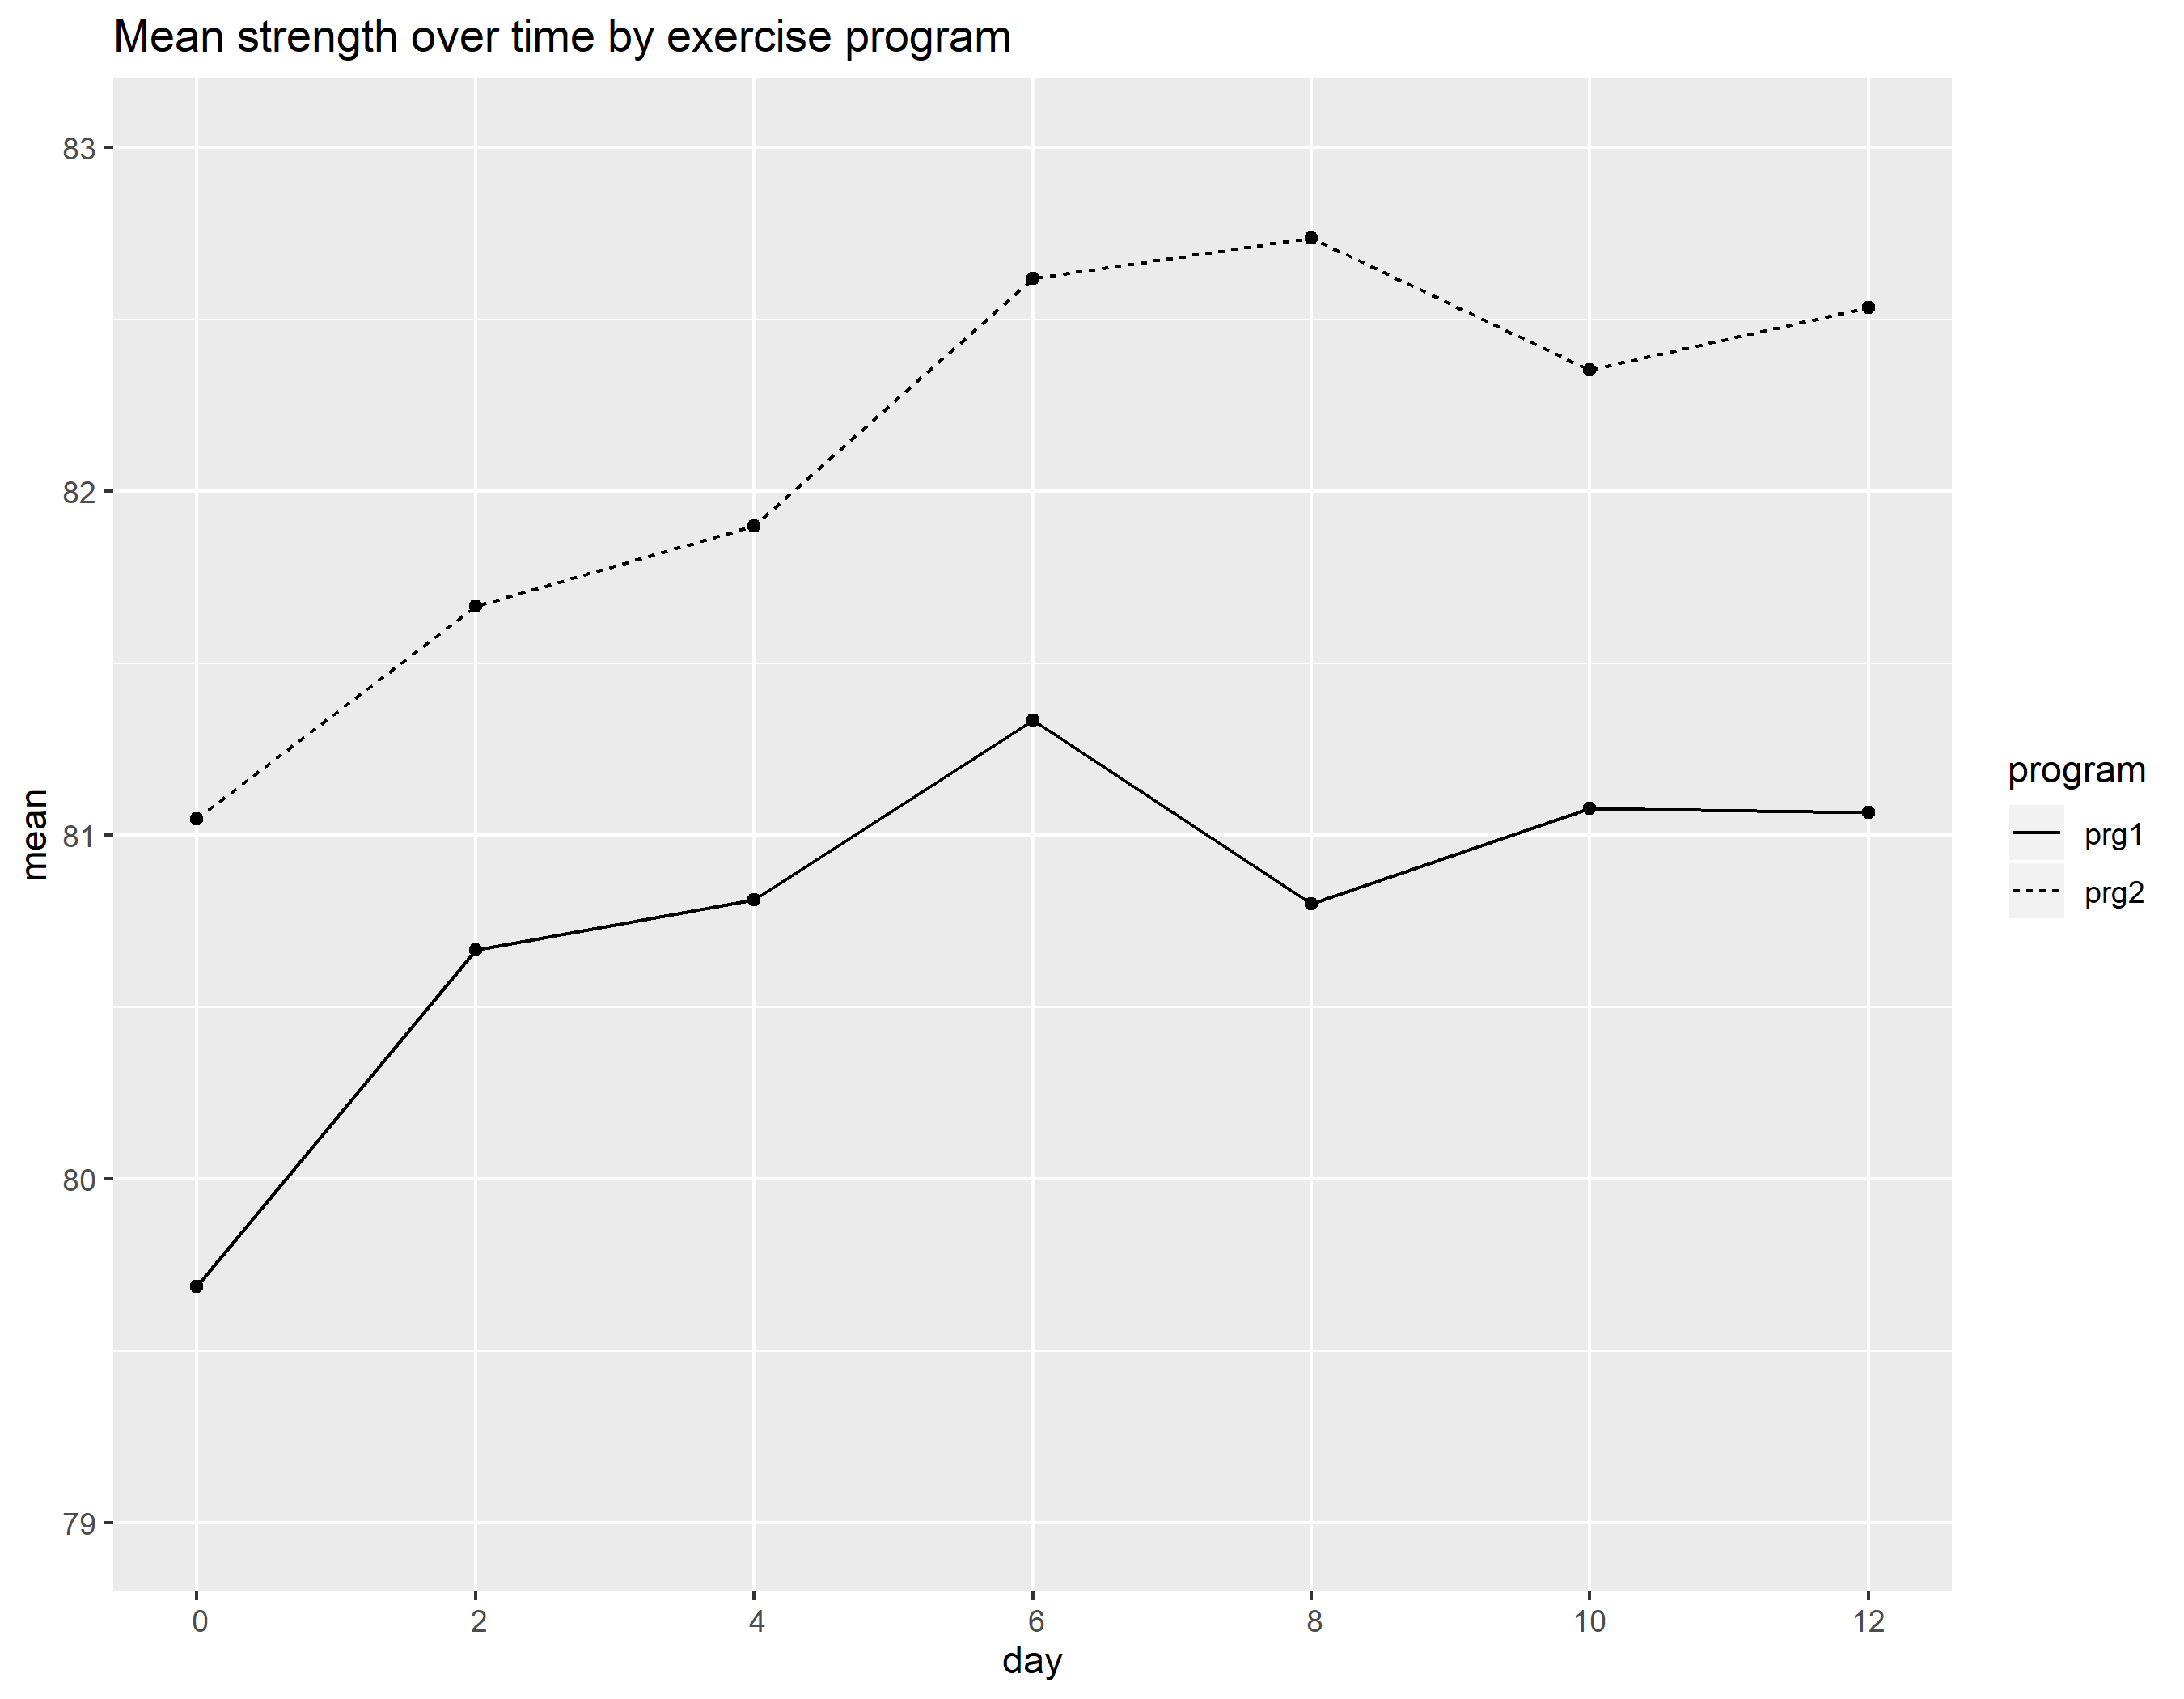
\includegraphics[scale=.4]{meanplot.png}\\
Looking at the graph we see that the mean strength tends to increase over time for both treatment groups. Treatment 1 decreases between day 6 and day 8, and for treatment 2, the mean strength decreases between day 8 and day 10. Treatment 2 has a higher mean strength than treatment 2 at baseline. The mean differences in strength over time between treatment 2 and treatment 1 are shown in the following table.\\
\begin{tabular}{cc}
	\hline
	day & $\mu_{diff}$ \\ 
	\hline
	0 & 1.36 \\ 
	2 & 1.00 \\ 
	4 & 1.09 \\ 
	6 & 1.29 \\ 
	8 & 1.94 \\ 
	10 & 1.28 \\ 
	12 & 1.47 \\ 
	\hline
\end{tabular}
\subsection*{Part 3}
$E(Y_{ij}|b_i)=\beta_1+b_{1i}+\beta_2 time+\beta_3 treatment1 +\beta_4 time*treatment1+b_{2i}time$\\
Where $time=(0,2,4,6,8,10,12)$ is the time in days when the measurement occurred\\
treatment1 is the indicator of the subject being in program 1
\begin{multline*}\\
\text{Estimated Regression Coefficients (fixed effects) and standard errors}\\
\begin{array}{ccc}
\hline
Parameter & estimate & se\\
\hline
\beta_1& 81.264 & .7\\
\beta_2& -.169 &.045\\
\beta_3&-1.131&1.064 \\
\beta_4&-.052&.067 \\
\hline
\end{array}\\
\end{multline*}
\begin{multline*}\\
\text{Estimated Covariance of the random effects and standard errors}\\
\begin{array}{ccc}
\hline
Parameter & estimate & se\\
\hline
Var(b_{1i})=g_{11}& 9.953& 2.457\\
Var(b_{2i})=g_{12}& -.017& .112 \\
Cov(b_{1i},b_{2i})=g_{22} &.034& .01\\
Var(\epsilon_i)=\sg^2_w& .665 & .073\\
\hline
\end{array}\\
\end{multline*}
\begin{enumerate}[(a)]
\item
Estimated variance of the random intercepts $= 9.953$
\item
Estimated variance of the random slopes $= .034$
\item
Estimated correlation between the random intercepts and
slopes $= -.029$
\item
$95\%$ CI baseline strength for program1\\
$(\hat{\beta_1}+ \hat{\beta_3})\pm \sqrt{g_{11}} =(73.949,86.315)$\\
$95\%$ CI baseline strength for program2\\ $\hat{\beta_1}\pm \sqrt{g_{11}} =(75.081,87.447)$\\
There is a large variability in the baseline strength in each program.\\
Approximately $95\%$ of the subjects in program 1 have a baseline strength between 73.949 and 86.315\\
Approximately $95\%$ of the subjects in program 2 have a baseline strength between 75.081 and 87.447\\
\item
$95\%$ CI change in baseline strength for program1\\ $(\hat{\beta_2}+\hat{\beta_4})\pm \sqrt{g_{22}}=(-.244,.478)$\\
Approximately $95\%$ of the subjects in program 1 have a change in strength between -.244 and .478\\
$95\%$ CI change in baseline strength for program2\\
$\hat{\beta_2}\pm \sqrt{g_{22}}=(-.192,.53)$\\
Approximately $95\%$ of the subjects in program 1 have a change in strength between -.192 and .53\\
There is a large variability in the change in baseline strength in each program.\\
\end{enumerate}
\pagebreak
\subsection*{Part 4}
LRT test comparing model with two random effects and model with one random effect using $\alpha=.05$\\
$H_0: g_{22}=0$\\
The critical value is a 50:50 mixture of chi-square distributions with 1 and 2 degrees of freedom\\
critical value $=5.14$\\
For the model with two random effects, $-2 log L = 818.5$\\
For the model with one random effect, $-2 log L=881.2$\\
$\chi^2_{obs}=881.2-818.5=62.7>5.14$ Reject $H_0$\\
Conclude there is significant evidence that the model with random slopes and random intercepts is a better
fit than the model with random intercepts only.
\subsection*{Part 5}
\begin{multline*}\\
\text{Mean intercept and  mean slope in each program}\\
\begin{array}{ccc}
\hline
Program &Intercept & Slope\\
\hline
1 & 80.132 & .117\\
2 & 81.263 & .169\\
\hline
\end{array}\\
\end{multline*}
\subsection*{Part 6}
From the table in the previous part, we see that the slope is .117 for program 1 and .169 for program 2. The estimated slope for program 2 is .052 units higher than for program 1.\\
This suggests that program 2 increases mean strength at higher rate than program 1.\\
Running a type 3 wald test on the interaction term\\
$H_0: \beta_4=0$\\
Wald $\chi^2_1=.59$ p-value$=.44>.05$ Fail to reject $H_0$, the interaction term is non significant\\
Thus conclude the changes in strength are not statistically significant between the two programs.
\subsection*{Part 7}
$\sg^2_w=.665$ \quad $\sg^2_b=9.953$\\
$Var(Y_{i1}|b_i)=\sg^2_w=.665$\\
$Var(Y_{i1})=\sg^2_w+\sg^2_b=.665+9.953=10.618$\\
The difference between the variance estimates is whether the estimate accounts for the between subject
variance. In this case, the between subject variance is a lot higher than the within subject variance.
\subsection*{Part 8}

\begin{tabular}{ccc}
\hline
&Empirical BLUP $b_i$\\
\hline
id & intercept & slope \\ 
\hline
1 & -1.052 & -0.077 \\ 
2 & 2.909 & 0.228 \\ 
3 & 1.642 & -0.034 \\ 
4 & 0.856 & -0.021 \\ 
5 & -0.001 & 0.264 \\ 
6 & -3.997 & -0.157 \\ 
7 & 1.963 & 0.150 \\ 
8 & -2.608 & 0.228 \\ 
9 & 5.125 & 0.065 \\ 
10 & -4.707 & 0.177 \\ 
11 & -3.390 & -0.140 \\ 
12 & 4.029 & 0.064 \\ 
13 & -1.199 & 0.110 \\ 
14 & -2.386 & -0.320 \\ 
15 & -1.583 & -0.404 \\ 
16 & 4.399 & -0.133 \\ 
17 & 2.690 & -0.213 \\ 
18 & -6.403 & -0.040 \\ 
19 & 1.407 & -0.189 \\ 
20 & 5.167 & -0.130 \\ 
21 & 1.234 & 0.103 \\ 
22 & -2.110 & -0.120 \\ 
23 & -2.610 & 0.172 \\ 
24 & 6.704 & 0.216 \\ 
25 & -0.547 & 0.022 \\ 
26 & 0.713 & 0.180 \\ 
27 & -2.171 & 0.051 \\ 
28 & -1.783 & 0.216 \\ 
29 & 2.253 & -0.146 \\ 
30 & -0.208 & 0.084 \\ 
31 & -3.124 & -0.092 \\ 
32 & 1.063 & -0.035 \\ 
33 & -1.787 & -0.097 \\ 
34 & -0.122 & -0.145 \\ 
35 & 4.292 & -0.102 \\ 
36 & -3.326 & 0.228 \\ 
37 & -1.332 & 0.035 \\ 
\hline
\end{tabular}\medbreak
In order to obtain the Predicted empirical BLUP intercept and slope estimates for each subject we must add the Mean intercept and  mean slope for the subjects respective program\\
\begin{tabular}{ccc}
	\hline
	&Predicted empirical BLUP intercept and slope\\
	\hline
	id & intercept & slope \\ 
	\hline
	1 & 79.080 & 0.040 \\ 
	2 & 83.041 & 0.345 \\ 
	3 & 81.774 & 0.083 \\ 
	4 & 80.989 & 0.096 \\ 
	5 & 80.131 & 0.381 \\ 
	6 & 76.135 & -0.040 \\ 
	7 & 82.095 & 0.267 \\ 
	8 & 77.524 & 0.345 \\ 
	9 & 85.257 & 0.182 \\ 
	10 & 75.425 & 0.294 \\ 
	11 & 76.742 & -0.023 \\ 
	12 & 84.161 & 0.181 \\ 
	13 & 78.933 & 0.227 \\ 
	14 & 77.746 & -0.203 \\ 
	15 & 78.549 & -0.287 \\ 
	16 & 84.531 & -0.016 \\ 
	17 & 83.953 & -0.044 \\ 
	18 & 74.860 & 0.129 \\ 
	19 & 82.670 & -0.020 \\ 
	20 & 86.430 & 0.039 \\ 
	21 & 82.497 & 0.272 \\ 
	22 & 79.153 & 0.049 \\ 
	23 & 78.654 & 0.342 \\ 
	24 & 87.967 & 0.385 \\ 
	25 & 80.716 & 0.191 \\ 
	26 & 81.976 & 0.349 \\ 
	27 & 79.092 & 0.220 \\ 
	28 & 79.480 & 0.385 \\ 
	29 & 83.516 & 0.024 \\ 
	30 & 81.055 & 0.253 \\ 
	31 & 78.139 & 0.077 \\ 
	32 & 82.326 & 0.134 \\ 
	33 & 79.476 & 0.072 \\ 
	34 & 81.141 & 0.024 \\ 
	35 & 85.555 & 0.067 \\ 
	36 & 77.937 & 0.397 \\ 
	37 & 79.931 & 0.204 \\ 
	\hline
\end{tabular}
\subsection*{Part 9}
\begin{tabular}{ccc}
\hline
&Subject 24 OLS Estimates\\	
\hline
Parameter & Estimate & se\\
\hline
Intercept & 87.8 & .787\\
Slope & .45 &.161\\
\hline
\end{tabular}
\subsection*{Part 10}
For subject 24, the empirical blup slope is .385 and the intercept is 87.967.\\
The empirical blup intercept is slightly higher but the OLS estimated slope is higher.\\
The empirical blup are predicted and the OLS estimates are estimated. A prediction usually has larger uncertainty than a related estimate, due to the added uncertainty in the outcome of that random variable. This is the main reason why the OLS estimates and the empirical BLUP differ.\\
Also for subject 24, two of the seven observations are missing which could effect the subjects predicted response.
\end{flushleft}
\end{document}
